%----------------------------------------------------------------------------------------
% HET SPREIDINGSDIAGRAM EN DE TRENDLIJN. Alle opgaven zijn eigen werk; alle gegevens zijn verzonnen.
%
% Opbouw: Probleem, Start, leerstof, en op een nieuwe pagina de Opdrachten en Test jezelf (geen Koppel in de 2de graad).
% Labels van dit hoofdstuk beginnen met h1-.
% Notatie zoals in Functies: rico m en vergelijking y = mx + q.
% Verschillen per pakket: residuen en de kleinste kwadraten (4-5), met een korte oefening en een opdracht;
% in de oefeningenbank een bewijsopdracht over de som van de residuen (5).
% Nagerekend (kleinste kwadraten): de ijsjes y = 11,78x - 122,72 met r = 0,97, gemiddelde punt (24, 160).
%----------------------------------------------------------------------------------------

\mychapter{1}{Het spreidingsdiagram en de trendlijn}

\begin{probleem}
Een ijskraam op de zeedijk noteert tien dagen lang de hoogste temperatuur $T$ van de dag (in °C) en het aantal verkochte ijsjes $N$. (De gegevens zijn verzonnen.)

\vspace{1mm}
{\centering\kleinetabel[$T$ (°C)][$N$]{10}{17 & 19 & 20 & 22 & 23 & 24 & 26 & 28 & 30 & 31}{85 & 89 & 125 & 120 & 165 & 145 & 180 & 225 & 221 & 245}\par}

\vspace{1mm}
Het weerbericht voorspelt voor morgen 27 °C. Hoeveel ijsjes moet de uitbater klaarzetten? Er was nog geen dag van 27 °C, en twee dagen met bijna dezelfde temperatuur (22 en 23 °C) verschillen wel 45 ijsjes. En wat kun je zeggen over een koude dag van 5 °C, of over een hittegolf van 40 °C?
\end{probleem}

\lkr{Leerplan \pakketnaam: LPD \alleenvoor{2}{34}\alleenvoor{3}{36}\alleenvoor{4,5}{40} (dit hoofdstuk: een spreidingsdiagram tekenen en lezen, een verband beschrijven, een trendlijn op het oog en met ICT, voorspellen, interpoleren en extrapoleren\alleenvoor{4,5}{, residuen en het idee van de kleinste kwadraten}). Het tweede hoofdstuk behandelt de correlatiecoëfficiënt. Voorkennis: de eerstegraadsfunctie $f(x) = mx + q$ uit Functies (rico met twee punten, voorschrift opstellen) en het gemiddelde; beide worden kort herhaald waar ze nodig zijn. Alle gegevens zijn verzonnen, maar realistisch gekozen. In de les volstaat een rekenmachine met een statistiekmodus voor twee variabelen; de knoppen verschillen per toestel, daarom beschrijft het boek de stappen in algemene termen. Toon in de les de knoppen van het toestel dat de school gebruikt. Laat de leerlingen bij het probleem eerst zelf een schatting maken: de meesten nemen iets tussen 180 en 225, het aantal bij 26 en 28 °C.}

Hoe hangt de verkoop van ijsjes af van het weer? Hoeveel duurder is een groter appartement? Bij zulke vragen meet je bij elke persoon, elke dag of elk ding twee getallen, en zoek je een verband. Een verband zoals in Functies, met één $y$ bij elke $x$, vind je daar zelden: de punten liggen niet netjes op een grafiek, maar vormen een wolk. In dit hoofdstuk leer je die wolk tekenen en lezen. Daarna trek je er een rechte door, de \textit{trendlijn}, eerst op het oog en dan met ICT. Met die rechte maak je voorspellingen, en je leert wanneer je die voorspellingen kunt vertrouwen.

\begin{oefeningen}[Start]
\oef{h1-start-1}

\oef{h1-verken}
\end{oefeningen}

%========================================================================================
\section{Het spreidingsdiagram}

\subsection{Twee variabelen tegelijk}

Een ijskraam noteert tien dagen lang de hoogste temperatuur $T$ (in °C) en het aantal verkochte ijsjes $N$. In Statistiek bekijk je telkens één variabele: de temperaturen, of het aantal ijsjes. Hier wil je weten hoe die twee samenhangen. Daarom horen bij elke dag twee getallen, die je samen bekijkt als een koppel $(T, N)$. De eerste dag geeft het koppel $(17, 85)$: 17 °C en 85 ijsjes. Zet je elk koppel als een punt in een assenstelsel, dan krijg je de figuur hiernaast.

\naast{In de tabel moet je lang zoeken. In de figuur zie je in één oogopslag dat het op warme dagen drukker is: hoe verder naar rechts, hoe hoger de punten liggen.

\vspace{1mm}
De temperatuur staat op de horizontale as: we willen het aantal ijsjes \textit{voorspellen uit} de temperatuur, en niet omgekeerd. Zoals bij functies staat de onafhankelijke variabele op de $x$-as en de afhankelijke op de $y$-as.

\vspace{1mm}
De $x$-as begint niet bij 0 maar bij 14: alle temperaturen liggen tussen 17 en 31 °C, en zo gebruik je de ruimte goed.}{\begin{tikzpicture}[x=.33cm,y=.0175cm]
  \diagram[$T$ (°C)][$N$ (ijsjes)]{14}{2}{34}{0}{20}{280}
  \xas{14,18,...,34}\yas{0,40,...,280}
  \punten{(17,85) (19,89) (20,125) (22,120) (23,165) (24,145) (26,180) (28,225) (30,221) (31,245)}
\end{tikzpicture}}

Er is één groot verschil met de grafiek van een functie. Twee dagen met dezelfde temperatuur kunnen een ander aantal ijsjes geven, want het aantal hangt ook af van de wind, de dag van de week en het toeval. De punten liggen dus niet op een mooie lijn, maar vormen samen een wolk.

\begin{theorie}
Meet je bij elk individu (een persoon, een dag, een land, \ldots) twee getallen $x$ en $y$, dan stelt een \textbf{\textcolor{accent}{spreidingsdiagram}} elk individu voor als een punt $\formule{(x, y)}$ in een assenstelsel. Alle punten samen heten de \textbf{\textcolor{accent}{puntenwolk}}.
\end{theorie}

Een spreidingsdiagram heeft geen lijn tussen de punten: elk punt is een aparte meting, en tussen twee dagen ligt geen ``halve dag''.

\voorbeeld{}{Acht leerlingen meten hun lengte $\ell$ en hun spanwijdte $s$: de afstand tussen de toppen van de middelvingers als ze de armen spreiden. Teken het spreidingsdiagram.

\vspace{1mm}
\waardetabel[$\ell$ (cm)][$s$ (cm)]{8}{158 & 162 & 165 & 168 & 171 & 175 & 178 & 184}{155 & 163 & 162 & 170 & 169 & 177 & 176 & 186}\label{vb:h1-tekenen}}{%
\naast{\uitleg{Hier is er geen echte oorzaak en gevolg. We zetten de lengte op de $x$-as, want die is gemakkelijker te meten: dan kun je de spanwijdte voorspellen uit de lengte. Daarna kiezen we de schaal.}
\begin{stappenvrij}{2.3cm}{5cm}
\ell:\ 158 \to 184 & De lengtes liggen tussen 158 en 184 cm: de $x$-as loopt van 150 tot 190, met een stap van 5. \\
s:\ 155 \to 186 & De spanwijdtes liggen tussen 155 en 186 cm: de $y$-as loopt ook van 150 tot 190. \\
(158, 155) & Per leerling één punt: eerst opzij tot 158, dan omhoog tot 155.
\end{stappenvrij}
\vspace{1mm}
De punten liggen dicht bij elkaar in een smalle, stijgende strook: wie groter is, heeft meestal een grotere spanwijdte, en die is ongeveer even groot als de lengte.}{\begin{tikzpicture}[x=.13cm,y=.13cm]
  \diagram[$\ell$ (cm)][$s$ (cm)]{150}{5}{190}{150}{5}{190}
  \xas{150,160,...,190}\yas{150,160,...,190}
  \punten{(158,155) (162,163) (165,162) (168,170) (171,169) (175,177) (178,176) (184,186)}
\end{tikzpicture}}}

\begin{werkwijze}
Kies welke variabele op de $x$-as komt: de variabele waarmee je de andere wilt verklaren of voorspellen. Zoek per as de kleinste en de grootste waarde, en kies een schaal met gelijke stappen die net iets ruimer is. Een as hoeft niet bij 0 te beginnen. Zet bij elke as de naam en de eenheid, en teken voor elk individu één punt, zonder lijnen ertussen.
\end{werkwijze}

\begin{oefeningen}
\oef{h1-tekenen}
\end{oefeningen}

\subsection{Een verband herkennen}

Wat kun je uit een puntenwolk aflezen? Kijk naar de vier spreidingsdiagrammen hieronder. In het eerste stijgen de punten van links naar rechts, zoals bij de ijsjes. In het tweede dalen ze. In het derde liggen ze kriskras door elkaar: kennen we $x$, dan weten we nog niets over $y$. In het vierde stijgen de punten eerst en dalen ze daarna: er is een duidelijk verband, maar de wolk volgt geen rechte.

\figuren{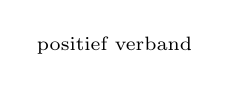
\begin{tikzpicture}[x=.3cm,y=.3cm,font=\scriptsize]
  \diagram{0}{2}{10}{0}{2}{10}
  \punten{(0.8,1.9) (1.6,1.7) (2.3,2.9) (2.9,3.9) (3.7,3) (4.4,4.2) (5.4,3.9) (6.5,5.2) (6.8,5) (7.5,6.7) (8.6,6.8) (9.3,8.4)}
  \node[below] at (5,-1.2) {positief verband};
\end{tikzpicture}\hfill
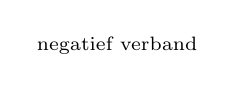
\begin{tikzpicture}[x=.3cm,y=.3cm,font=\scriptsize]
  \diagram{0}{2}{10}{0}{2}{10}
  \punten{(0.8,8.3) (1.6,7.5) (2.3,5.4) (2.9,6.4) (3.7,6.2) (4.4,5.8) (5.4,3.9) (6.5,3.9) (6.8,3.4) (7.5,3) (8.6,3.5) (9.3,1.7)}
  \node[below] at (5,-1.2) {negatief verband};
\end{tikzpicture}\hfill
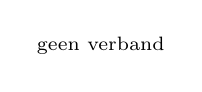
\begin{tikzpicture}[x=.3cm,y=.3cm,font=\scriptsize]
  \diagram{0}{2}{10}{0}{2}{10}
  \punten{(0.8,1.5) (1.6,7.3) (2.3,2.6) (2.9,3.4) (3.7,7.7) (4.4,5.1) (5.4,7.4) (6.5,6) (6.8,6.7) (7.5,2.1) (8.6,5.3) (9.3,5.1)}
  \node[below] at (5,-1.2) {geen verband};
\end{tikzpicture}\hfill
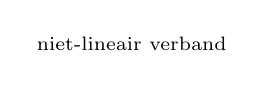
\begin{tikzpicture}[x=.3cm,y=.3cm,font=\scriptsize]
  \diagram{0}{2}{10}{0}{2}{10}
  \punten{(0.8,3.3) (1.6,6) (2.3,6.9) (2.9,7.1) (3.7,8.3) (4.4,8.9) (5.4,8.7) (6.5,8.4) (6.8,7.8) (7.5,7.2) (8.6,5.4) (9.3,3)}
  \node[below] at (5,-1.2) {niet-lineair verband};
\end{tikzpicture}}

Eerst geven we de richting van een verband een naam.

\begin{theorie}
Twee variabelen hebben een \textbf{\textcolor{accent}{positief verband}} als bij een grotere $x$ meestal een grotere $y$ hoort: de puntenwolk stijgt.

\vspace{1mm}
Ze hebben een \textbf{\textcolor{accent}{negatief verband}} als bij een grotere $x$ meestal een kleinere $y$ hoort: de puntenwolk daalt.
\end{theorie}

Het woord ``meestal'' is belangrijk: niet elk punt hoeft hoger te liggen dan het punt links ervan. Bij de ijsjes verkocht de dag van 23 °C meer dan de dag van 24 °C, en toch is het verband positief. Je kijkt naar de wolk als geheel. Positief en negatief zijn hier dus geen woorden voor goed en slecht: minder ongevallen bij meer verlichting is een negatief verband.

Naast de richting heeft een verband ook een vorm.

\begin{theorie}
Een verband is \textbf{\textcolor{accent}{lineair}} als de punten van de puntenwolk ongeveer op een rechte liggen.
\end{theorie}

In het vierde diagram hierboven is het verband niet lineair: de punten volgen een boog. In dit boek werken we verder met lineaire verbanden. Bij een lineair verband zeg je ook hoe \textit{sterk} het is: hoe dichter de punten bij een rechte liggen, hoe sterker het verband. In de twee diagrammen hieronder is het verband positief en lineair, maar links is het veel sterker dan rechts. In het volgende hoofdstuk druk je die sterkte uit met een getal.

\figuren{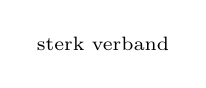
\begin{tikzpicture}[x=.3cm,y=.3cm,font=\scriptsize]
  \diagram{0}{2}{10}{0}{2}{10}
  \punten{(0.8,2.1) (1.6,2.5) (2.3,3.1) (2.9,3.2) (3.7,3.9) (4.4,4.5) (5.4,5.5) (6.5,6.4) (6.8,5.9) (7.5,6.5) (8.6,7.7) (9.3,7.4)}
  \node[below] at (5,-1.2) {sterk verband};
\end{tikzpicture}\qquad\qquad
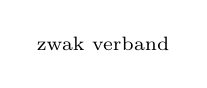
\begin{tikzpicture}[x=.3cm,y=.3cm,font=\scriptsize]
  \diagram{0}{2}{10}{0}{2}{10}
  \punten{(0.8,2.4) (1.6,4.4) (2.3,6.8) (2.9,5.2) (3.7,2.9) (4.4,4.2) (5.4,6.8) (6.5,8.2) (6.8,4.2) (7.5,5.7) (8.6,8.2) (9.3,5.8)}
  \node[below] at (5,-1.2) {zwak verband};
\end{tikzpicture}}

Soms ligt één punt ver van de rest van de wolk. Zo'n punt heet een \emph{uitschieter}. Kijk dan na of het geen meetfout of tikfout is. Is het een echte meting, dan hoort het erbij, maar vermeld je het apart: het kan een bijzonder geval zijn dat de moeite waard is.

\voorbeeld{}{Een garage verkoopt elf tweedehandswagens van hetzelfde merk. Het spreidingsdiagram toont de leeftijd $a$ (in jaar) en de prijs $p$ (in duizend euro) van elke wagen. Beschrijf het verband.\label{vb:h1-verband}}{%
\naast{\uitleg{We bekijken achtereenvolgens de richting, de vorm, de sterkte en de uitschieters.}
\begin{stappenvrij}{1.9cm}{5.8cm}
\text{richting} & Hoe ouder de wagen, hoe lager meestal de prijs: een negatief verband. \\
\text{vorm} & Op één punt na liggen de punten ongeveer op een dalende rechte: lineair. \\
\text{sterkte} & De punten liggen dicht bij die rechte: een sterk verband. \\
\text{uitschieter} & De wagen van 9 jaar kost 22\,000 euro, veel meer dan de rest van zijn leeftijd.
\end{stappenvrij}
\vspace{1mm}
Misschien is die wagen een zeldzame uitvoering, of is de prijs fout ingetikt. Dat moet de garage nakijken.}{\begin{tikzpicture}[x=.5cm,y=.17cm]
  \diagram[$a$ (jaar)][$p$ (duizend euro)]{0}{1}{11}{0}{2}{26}
  \xas{0,2,...,10}\yas{0,4,...,24}
  \punten{(1,24) (2,21) (3,20) (3,18) (4,16) (5,15) (6,12) (7,11) (8,8) (9,22) (10,6)}
  \draw[inkt,thick] (9,22) circle (5pt);
\end{tikzpicture}}}

\begin{werkwijze}
Beschrijf een verband in vier stappen. Richting: stijgt de wolk (positief), daalt ze (negatief), of geen van beide (geen verband)? Vorm: liggen de punten ongeveer op een rechte (lineair) of niet? Sterkte: liggen ze dicht bij die rechte (sterk) of ver ervan (zwak)? Uitschieters: is er een punt dat ver van de rest ligt?
\end{werkwijze}

\begin{oefeningen}
\needspace{16\baselineskip}
\oef{h1-verband}
\end{oefeningen}

%========================================================================================
\section{De trendlijn}

\subsection{Een rechte door de puntenwolk}

Hoeveel ijsjes verkoopt het ijskraam bij 25 °C? Er was geen dag van 25 °C, en de dagen van 24 en 26 °C verschillen 35 ijsjes. Het verband is lineair, dus een goed idee is: trek een rechte die de puntenwolk zo goed mogelijk volgt, en lees de voorspelling op die rechte af. Door alle punten gaat ze niet, want de punten liggen niet op één rechte. Maar ze kan wel zo lopen dat de punten er aan beide kanten dicht bij liggen.

\begin{theorie}
Een \textbf{\textcolor{accent}{trendlijn}} is een rechte die de richting van een puntenwolk zo goed mogelijk volgt. Zoals elke rechte die niet verticaal is, heeft ze een vergelijking

\vspace{1mm}
\qquad $\formule{y = mx + q}$
\end{theorie}

Uit Functies weet je wat $m$ en $q$ betekenen: $m$ is de richtingscoëfficiënt (de rico) en $(0, q)$ is het snijpunt met de $y$-as. Gaat een rechte door twee punten $(x_1, y_1)$ en $(x_2, y_2)$, dan is $m = \tfrac{y_2 - y_1}{x_2 - x_1}$. Het getal $q$ vind je daarna door één punt in te vullen in $y = mx + q$.

Hoe trek je zo'n rechte op het oog? Een goed houvast is het \textit{gemiddelde punt} $(\xbar, \ybar)$: het punt met als coördinaten het gemiddelde van alle $x$-waarden en het gemiddelde van alle $y$-waarden. Dat punt ligt midden in de wolk. Een trendlijn door het gemiddelde punt laat ongeveer evenveel punten boven als onder zich, en de punten erboven compenseren de punten eronder.

\voorbeeld{}{Teken op het oog een trendlijn door de puntenwolk van de ijsjes, en stel haar vergelijking op.\label{vb:h1-trendoog}}{%
\naast{\uitleg{We berekenen eerst het gemiddelde punt. Daarna draaien we een lat rond dat punt tot ze de wolk goed volgt, en lezen we een tweede punt van de rechte af op een kruispunt van het rooster.}
\begin{stappenvrij}{3.7cm}{4.6cm}
\xbar = \frac{240}{10} = 24 & De som van de tien temperaturen, gedeeld door 10. \\
\ybar = \frac{1600}{10} = 160 & De som van de aantallen ijsjes, gedeeld door 10. \\
(24, 160) \text{ en } (16, 60) & Het gemiddelde punt en een tweede punt van de getekende rechte. \\
m = \frac{160 - 60}{24 - 16} = 12,5 & De rico met twee punten. \\
160 = 12,5 \cdot 24 + q & Vul het gemiddelde punt in. \\
q = 160 - 300 = -140 &
\end{stappenvrij}}{\begin{tikzpicture}[x=.26cm,y=.016cm]
  \diagram[$T$ (°C)][$N$ (ijsjes)]{14}{2}{34}{0}{20}{280}
  \xas{14,18,...,34}\yas{0,40,...,280}
  \rechte{14}{33.6}{12.5}{-140}
  \punten{(17,85) (19,89) (20,125) (22,120) (23,165) (24,145) (26,180) (28,225) (30,221) (31,245)}
  \gempunt{24}{160}
  \punt[inkt]{16}{60}
  \node[right,font=\scriptsize,text=inkt] at (24,155) {$(\xbar, \ybar)$};
\end{tikzpicture}}
\vspace{1mm}
De trendlijn is $N = 12,5\,T - 140$. Vier punten liggen erboven en zes eronder, maar die zes liggen er gemiddeld dichter bij: samen wijken de punten erboven evenveel af als de punten eronder. Een klasgenoot die de lat iets anders legt, vindt bijvoorbeeld $N = 12\,T - 128$: op het oog is er niet één juist antwoord, wel een strook van goede antwoorden.}

\begin{werkwijze}
Bereken het gemiddelde punt $(\xbar, \ybar)$ en duid het aan. Leg een lat door dat punt en draai ze tot ze de richting van de wolk volgt, met ongeveer evenveel punten aan elke kant. Trek de rechte en lees er een tweede punt op af, liefst op een kruispunt van het rooster en ver van het gemiddelde punt. Bereken $m$ met de twee punten, en $q$ door een punt in te vullen in $y = mx + q$.
\end{werkwijze}

\nujij{Een trendlijn gaat door het gemiddelde punt $(10, 50)$ en door $(20, 80)$. Geef haar vergelijking.}{$m = \tfrac{80 - 50}{20 - 10} = 3$ en $50 = 3 \cdot 10 + q$, dus $q = 20$: $y = 3x + 20$.}

\begin{oefeningen}
\oef{h1-trendoog}
\end{oefeningen}

\subsection{Wat zeggen $m$ en $q$?}

Een trendlijn is meer dan een hulpmiddel om af te lezen. Haar rico en haar snijpunt met de $y$-as vertellen iets over de situatie. Bij een eerstegraadsfunctie zegt de rico hoeveel $y$ verandert als $x$ met 1 toeneemt. Bij een trendlijn is dat net zo, maar dan ``gemiddeld'' of ``ongeveer'': de punten liggen niet precies op de rechte.

\voorbeeld{}{Wat betekenen de getallen $12,5$ en $-140$ in de trendlijn $N = 12,5\,T - 140$ van de ijsjes?\label{vb:h1-betekenis}}{%
\uitleg{De rico is de verandering van $N$ als $T$ met 1 toeneemt. Het getal $q$ is de waarde van $N$ als $T = 0$.}
\begin{stappen}
m = 12,5 & Per graad warmer verkoopt de kraam gemiddeld ongeveer 12,5 ijsjes meer. \\
q = -140 & Bij 0 °C zou de kraam $-140$ ijsjes verkopen.
\end{stappen}
Een negatief aantal ijsjes kan niet. Het getal $q$ is hier alleen een rekenhulp om de rechte vast te leggen: de kleinste temperatuur in de tabel is 17 °C, en of het verband bij 0 °C nog zo verloopt, weten we niet. In de laatste sectie komen we daarop terug.}

Het getal $q$ heeft dus alleen een betekenis als $x = 0$ een zinvolle waarde is die bij de gegevens past. Bij een trendlijn voor de huurprijs van een appartement in functie van de oppervlakte is een appartement van 0 m² zinloos. Bij de prijs van een wagen in functie van zijn leeftijd is $q$ wel zinvol: dat is ongeveer de prijs van een nieuwe wagen.

\begin{oefeningen}
\oef{h1-betekenis}
\end{oefeningen}

\subsection{Voorspellen met de trendlijn}

Met de vergelijking van de trendlijn hoef je niet meer af te lezen: je rekent de voorspelling uit. Je kunt ook omgekeerd werken en een vergelijking oplossen.

\voorbeeld{}{Gebruik de trendlijn $N = 12,5\,T - 140$. Hoeveel ijsjes verwacht je bij 21 °C? Vanaf welke temperatuur verwacht je meer dan 200 ijsjes?\label{vb:h1-voorspel}}{%
\uitleg{Voor de eerste vraag vullen we $T = 21$ in. Voor de tweede kennen we $N$ en zoeken we $T$: dat is een eerstegraadsvergelijking.}
\begin{stappen}
N = 12,5 \cdot 21 - 140 = 122,5 & Vul $T = 21$ in: ongeveer 120 ijsjes. \\
12,5\,T - 140 = 200 & Wanneer is $N$ gelijk aan 200? \\
12,5\,T = 340 \quad\Longrightarrow\quad T = 27,2 & Tel 140 op, en deel door 12,5.
\end{stappen}
Bij 21 °C verwacht je ongeveer 120 ijsjes, en vanaf ongeveer 27 °C meer dan 200. Een voorspelling is een schatting: rond haar af, want de echte dagen wijken tot bijna 20 ijsjes af van de trendlijn.}

\begin{oefeningen}
\oef{h1-voorspel}
\end{oefeningen}

%========================================================================================
\section{De regressielijn}

Op het oog vindt iedereen een iets andere trendlijn, en dus een iets andere voorspelling. Voor de uitbater van het ijskraam maakt dat weinig uit, maar wie twee onderzoeken wil vergelijken, wil één afgesproken trendlijn. Welke rechte is de beste?

\begin{alleenvoor}{2,3}
Je rekenmachine en een rekenblad kunnen die beste rechte berekenen. Ze kijken voor elke rechte hoe ver de punten er boven of onder liggen, en kiezen de rechte waarbij de punten samen zo weinig mogelijk afwijken. Hoe ze die afwijkingen precies samentellen, hoef je niet te kennen.
\end{alleenvoor}
\begin{alleenvoor}{4,5}
\subsection{Residuen en de kleinste kwadraten}

Om rechten te vergelijken, meten we hoe ver elk punt van de rechte ligt. We meten verticaal, want we gebruiken de rechte om $y$ te voorspellen: de afwijking is het verschil tussen de echte $y$ en de voorspelde.

\begin{theorie}
Het \textbf{\textcolor{accent}{residu}} van een punt $(x, y)$ tegenover de rechte $y = mx + q$ is

\vspace{1mm}
\qquad $\formule{\text{residu} = y - (mx + q)}$

\vspace{1mm}
Het residu is positief als het punt boven de rechte ligt en negatief als het eronder ligt.
\end{theorie}

Kunnen we de residuen gewoon optellen? Nee: positieve en negatieve residuen heffen elkaar op. Voor elke rechte door het gemiddelde punt is de som van de residuen zelfs 0, hoe scheef de rechte ook staat. Daarom kwadrateren we de residuen eerst: een kwadraat is nooit negatief, en een groot residu weegt extra zwaar door.

\voorbeeld{}{Gegeven zijn de punten $(1, 2)$, $(2, 3)$, $(3, 5)$ en $(4, 6)$. Welke rechte past het best: $a\colon y = x + 1,5$ of $b\colon y = 1,4x + 0,5$? Vergelijk de som van de kwadraten van de residuen.\label{vb:h1-residu}}{%
\naast{\uitleg{Beide rechten gaan door het gemiddelde punt $(2,5;\ 4)$. We berekenen per punt het residu, kwadrateren en tellen op.}

\vspace{1mm}
{\renewcommand{\arraystretch}{1.3}\small\begin{tabular}{|c|c|c|c|c|}\hline
punt & $a$: residu & kwadraat & $b$: residu & kwadraat \\ \hline
$(1, 2)$ & $2 - 2,5 = -0,5$ & $0,25$ & $2 - 1,9 = 0,1$ & $0,01$ \\
$(2, 3)$ & $3 - 3,5 = -0,5$ & $0,25$ & $3 - 3,3 = -0,3$ & $0,09$ \\
$(3, 5)$ & $5 - 4,5 = 0,5$ & $0,25$ & $5 - 4,7 = 0,3$ & $0,09$ \\
$(4, 6)$ & $6 - 5,5 = 0,5$ & $0,25$ & $6 - 6,1 = -0,1$ & $0,01$ \\ \hline
som & $0$ & $1$ & $0$ & $0,2$ \\ \hline
\end{tabular}}}{\begin{tikzpicture}[x=.7cm,y=.55cm]
  \rooster{0}{1}{5}{0}{1}{7}
  \rechte[tweede]{0.3}{5}{1}{1.5}
  \rechte{0.3}{5}{1.4}{0.5}
  \residu{1}{2}{1.4}{0.5}\residu{2}{3}{1.4}{0.5}\residu{3}{5}{1.4}{0.5}\residu{4}{6}{1.4}{0.5}
  \punten{(1,2) (2,3) (3,5) (4,6)}
  \node[right,font=\scriptsize,text=inkt] at (5,6.5) {$a$};
  \node[right,font=\scriptsize] at (4.6,7) {$b$};
\end{tikzpicture}}
\vspace{1mm}
De sommen van de residuen zijn allebei 0, dus die zeggen niets. De som van de kwadraten is bij $b$ vijf keer kleiner: rechte $b$ past het best. Ze is zelfs de beste van alle rechten, zoals ICT bevestigt.}

\begin{theorie}
De \textbf{\textcolor{accent}{regressielijn}} is de rechte waarvoor de som van de kwadraten van de residuen het kleinst is. Daarom heet ze ook de \textbf{\textcolor{accent}{kleinste-kwadratenlijn}}.

\begin{stelling}{Gemiddelde punt}
De regressielijn gaat door het gemiddelde punt $\formule{(\xbar, \ybar)}$.
\end{stelling}
\end{theorie}

Waarom die eigenschap klopt, bewijzen we niet: dat vraagt meer algebra dan we nu hebben. Je kunt ze wel telkens nagaan, en ze verklaart waarom een trendlijn op het oog door het gemiddelde punt een goede keuze is. Met de hand de beste rechte zoeken is veel werk, want er zijn oneindig veel rechten door het gemiddelde punt. Dat laten we over aan ICT.

\begin{oefeningen}
\oef{h1-residu}
\end{oefeningen}
\end{alleenvoor}

\begin{alleenvoor}{2,3}
\begin{theorie}
De \textbf{\textcolor{accent}{regressielijn}} is de trendlijn die ICT berekent: de rechte waarbij de punten samen het minst afwijken.

\begin{stelling}{Gemiddelde punt}
De regressielijn gaat door het gemiddelde punt $\formule{(\xbar, \ybar)}$.
\end{stelling}
\end{theorie}

Die eigenschap bewijzen we niet, maar je kunt ze telkens nagaan. Ze verklaart waarom een trendlijn op het oog door het gemiddelde punt een goede keuze is.
\end{alleenvoor}

\subsection{De regressielijn met ICT}

Elke wetenschappelijke of grafische rekenmachine met een statistiekmodus berekent de regressielijn, en ook elk rekenblad. De knoppen verschillen per toestel, maar de stappen zijn overal dezelfde.

\voorbeeld{}{Bereken met ICT de regressielijn van de ijsjes. Vergelijk ze met de trendlijn op het oog, $N = 12,5\,T - 140$.\label{vb:h1-ict}}{%
\naast{\uitleg{We voeren de tien temperaturen in als eerste lijst en de tien aantallen als tweede lijst, in dezelfde volgorde, en vragen de lineaire regressie.}
\begin{stappenvrij}{4.2cm}{4.1cm}
m = 11,78 & De rico die het toestel geeft. \\
q = -122,72 & Het snijpunt met de $y$-as. \\
N = 11,78\,T - 122,72 & De regressielijn. \\
11,78 \cdot 24 - 122,72 = 160 & Controle met het gemiddelde punt.
\end{stappenvrij}}{\begin{tikzpicture}[x=.26cm,y=.016cm]
  \diagram[$T$ (°C)][$N$ (ijsjes)]{14}{2}{34}{0}{20}{280}
  \xas{14,18,...,34}\yas{0,40,...,280}
  \rechte[tweede]{14}{33.6}{12.5}{-140}
  \rechte{14}{34}{11.78}{-122.72}
  \punten{(17,85) (19,89) (20,125) (22,120) (23,165) (24,145) (26,180) (28,225) (30,221) (31,245)}
  \gempunt{24}{160}
\end{tikzpicture}}
\vspace{1mm}
De regressielijn (volle lijn) is iets minder steil dan de trendlijn op het oog (streepjes), maar het verschil is klein. Bij 25 °C geeft de trendlijn op het oog $12,5 \cdot 25 - 140 = 172,5$ ijsjes, de regressielijn $11,78 \cdot 25 - 122,72 \approx 172$.}

\begin{werkwijze}
Zet de rekenmachine in de statistiekmodus voor twee variabelen (die heet soms ``lineaire regressie'' of ``$a + bx$''). Voer de $x$-waarden in een eerste lijst in en de bijbehorende $y$-waarden in een tweede, in dezelfde volgorde. Vraag de lineaire regressie: je krijgt de rico en het snijpunt met de $y$-as. Kijk goed welke letter de rico is, want sommige toestellen schrijven $y = ax + b$ en andere $y = a + bx$. Rond af en schrijf de vergelijking als $y = mx + q$. Controleer met het gemiddelde punt. In een rekenblad maak je een spreidingsdiagram en voeg je een lineaire trendlijn toe met haar vergelijking.
\end{werkwijze}

Hoe ver rond je af? Behoud genoeg cijfers om de voorspellingen niet te bederven: twee cijfers na de komma is meestal genoeg. Is de rico erg klein, zoals $-0,0062$ graden per meter, dan rond je niet af tot $-0,01$, maar kies je beter een andere eenheid: $-6,2$ graden per kilometer.

\begin{oefeningen}
\oef{h1-ict}
\end{oefeningen}

%========================================================================================
\section{Interpoleren en extrapoleren}

Mag je de regressielijn van de ijsjes gebruiken voor elke temperatuur? Probeer 8 °C: $N = 11,78 \cdot 8 - 122,72 \approx -28$. Een negatief aantal ijsjes is onzin. Wat ging er mis? De gegevens lagen allemaal tussen 17 en 31 °C. Daar volgen de punten een rechte, maar niemand heeft gemeten wat er bij 8 °C gebeurt. Waarschijnlijk verkoopt de kraam dan nog een paar ijsjes, en buigt de wolk daar af naar een horizontale lijn net boven 0.

\begin{theorie}
De gegevens van $x$ liggen tussen de kleinste en de grootste waarde. Een voorspelling voor een $x$ binnen dat gebied heet \textbf{\textcolor{accent}{interpoleren}}. Een voorspelling voor een $x$ erbuiten heet \textbf{\textcolor{accent}{extrapoleren}}.
\end{theorie}

Bij interpoleren steun je op gegevens aan beide kanten, en is de voorspelling meestal betrouwbaar. Bij extrapoleren veronderstel je dat het verband buiten de gegevens even recht blijft doorlopen. Dat is een gok: een beetje buiten het gebied kan het meevallen, ver erbuiten gaat het bijna altijd mis.

\voorbeeld{}{Noor werd elk jaar op haar verjaardag gemeten, van 2 tot 10 jaar. De regressielijn van haar lengte $\ell$ (in cm) in functie van haar leeftijd $a$ (in jaar) is $\ell = 6,45\,a + 75,52$. Hoe groot was ze op 6,5 jaar? Hoe groot zal ze zijn op 30 jaar?\label{vb:h1-extrapoleren}}{%
\naast{\uitleg{De leeftijden liggen tussen 2 en 10 jaar. 6,5 jaar ligt erbinnen (interpoleren), 30 jaar ver erbuiten (extrapoleren).}
\begin{stappenvrij}{3.8cm}{3.5cm}
6,45 \cdot 6,5 + 75,52 \approx 117 & Op 6,5 jaar: ongeveer 117 cm. \\
6,45 \cdot 30 + 75,52 \approx 269 & Op 30 jaar: 2,69 m?
\end{stappenvrij}
\vspace{1mm}
De eerste voorspelling is betrouwbaar: de metingen op 6 en 7 jaar waren 115 en 122 cm. De tweede is onzin. Rond 16 à 18 jaar stopt een mens met groeien: de grafiek buigt af en wordt horizontaal. Het verband is alleen lineair tussen 2 en 10 jaar.}{\begin{tikzpicture}[x=.2cm,y=.018cm]
  \diagram[$a$ (jaar)][$\ell$ (cm)]{0}{2}{32}{60}{20}{280}
  \xas{0,10,20,30}\yas{60,100,...,260}
  \rechte[tweede]{10}{32}{6.45}{75.52}
  \rechte{0}{10}{6.45}{75.52}
  \kromme[hulplijn]{10}{32}{170-32*exp(-(\x-10)/3.2)}
  \punten{(2,86) (3,95) (4,102) (5,109) (6,115) (7,122) (8,128) (9,133) (10,138)}
  \node[font=\scriptsize,text=inkt,anchor=east] at (25,250) {regressielijn};
  \node[font=\scriptsize,text=grijs,anchor=west] at (19,155) {echte groei};
\end{tikzpicture}}}

\begin{werkwijze}
Kijk vóór je voorspelt tussen welke waarden de gegevens van $x$ liggen. Ligt de nieuwe $x$ daartussen, dan interpoleer je, en is de voorspelling meestal betrouwbaar. Ligt ze erbuiten, dan extrapoleer je: vermeld dat, en vraag je af of het verband daar nog lineair kan zijn. Een onmogelijke uitkomst, zoals een negatief aantal of een te grote lengte, wijst altijd op een te verre extrapolatie.
\end{werkwijze}

\begin{oefeningen}
\oef{h1-interextra}
\end{oefeningen}

\voorbeeld{}{Terug naar het probleem. Een ijskraam op de zeedijk noteerde tien dagen lang de hoogste temperatuur $T$ (in °C) en het aantal verkochte ijsjes $N$.

\vspace{1mm}
{\centering\kleinetabel[$T$ (°C)][$N$]{10}{17 & 19 & 20 & 22 & 23 & 24 & 26 & 28 & 30 & 31}{85 & 89 & 125 & 120 & 165 & 145 & 180 & 225 & 221 & 245}\par}

\vspace{1mm}
Het weerbericht voorspelt voor morgen 27 °C. Hoeveel ijsjes moet de uitbater klaarzetten? Wat kun je zeggen over een koude dag van 5 °C en over een hittegolf van 40 °C?\label{vb:h1-terug}}{%
\uitleg{De regressielijn van deze gegevens is $N = 11,78\,T - 122,72$ (voorbeeld \ref{vb:h1-ict}). We gebruiken ze en kijken telkens of we interpoleren of extrapoleren. De gegevens lopen van 17 tot 31 °C.}
\begin{stappenbreed}
N = 11,78 \cdot 27 - 122,72 \approx 195 & 27 °C ligt tussen 17 en 31 °C: interpoleren. \\
N = 11,78 \cdot 5 - 122,72 \approx -64 & 5 °C ligt ver onder 17 °C: extrapoleren, en de uitkomst is onmogelijk. \\
N = 11,78 \cdot 40 - 122,72 \approx 348 & 40 °C ligt boven 31 °C: extrapoleren.
\end{stappenbreed}
\figuren{\begin{tikzpicture}[x=.3cm,y=.0105cm,font=\scriptsize]
  \diagram[$T$ (°C)][$N$ (ijsjes)]{0}{2}{42}{-80}{40}{360}
  \xas{0,5,...,40}\yas{-80,0,80,...,320}
  \fill[accent!8] (17,-80) rectangle (31,360);
  \draw[black!14,very thin,xstep=2,ystep=40] (0,-80) grid (42,360);
  \draw[grijs] (0,0) -- (42,0);
  \rechte{17}{31}{11.78}{-122.72}
  \rechte[densely dashed]{3.6}{17}{11.78}{-122.72}
  \rechte[densely dashed]{31}{41.5}{11.78}{-122.72}
  \punten{(17,85) (19,89) (20,125) (22,120) (23,165) (24,145) (26,180) (28,225) (30,221) (31,245)}
  \foreach \t/\n in {5/-63.8,27/195.3,40/348.5}{\filldraw[inkt,fill=white,thick] (\t,\n) circle (2.4pt);}
  \node[anchor=north,text=accent] at (24,355) {gegevens};
  \node[anchor=west,text=inkt] at (5.6,-63.8) {$-64$};
  \node[anchor=east,text=inkt] at (26.4,195.3) {$195$};
  \node[anchor=east,text=inkt] at (39.4,348.5) {$348$};
\end{tikzpicture}}
Het gekleurde deel toont de gegevens: daarbinnen interpoleer je, daarbuiten (de streepjes) extrapoleer je. Bij 27 °C verwacht de uitbater ongeveer 195 ijsjes. De echte dagen wijken tot bijna 20 ijsjes af van de regressielijn: met ongeveer 215 ijsjes heeft hij genoeg. Over 5 °C zeggen de gegevens niets, behalve dat het weinig zal zijn. Ook 348 ijsjes bij 40 °C is onzeker: misschien blijven de mensen bij die hitte thuis, en dan daalt de verkoop. Om dat te weten, heb je metingen bij zulke temperaturen nodig.}

%========================================================================================
\opdrachtenkop

\begin{oefeningen}
\oef{h1-o1}

\oef{h1-o2}

\oef{h1-o3}

\needspace{11\baselineskip}
\oef{h1-o4}

\needspace{11\baselineskip}
\oef{h1-o5}

\oef{h1-o6}

\oef{h1-o7}

\oef{h1-o8}

\needspace{11\baselineskip}
\oef{h1-o9}

\needspace{11\baselineskip}
\oef{h1-o10}

\needspace{11\baselineskip}
\oef{h1-o11}

\needspace{11\baselineskip}
\oef{h1-o12}

\oef{h1-o13}

\needspace{11\baselineskip}
\oef{h1-o14}

\needspace{11\baselineskip}
\oef{h1-o15}

\needspace{11\baselineskip}
\oef{h1-o16}

\needspace{16\baselineskip}
\oef{h1-o17}

\oef{h1-o18}

\oef{h1-o19}

\oef{h1-o20}

\needspace{11\baselineskip}
\oef{h1-o21}

\needspace{11\baselineskip}
\oef{h1-o22}

\needspace{11\baselineskip}
\oef{h1-o23}

\oef{h1-o24}

\oef{h1-o25}
\end{oefeningen}

%----------------------------------------------------------------------------------------
\opdrachtsectie{Test jezelf}

\begin{oefeningen}
\needspace{11\baselineskip}
\oef{h1-t1}

\oef{h1-t2}

\needspace{11\baselineskip}
\oef{h1-t3}

\oef{h1-t4}

\needspace{11\baselineskip}
\oef{h1-t5}

\oef{h1-t6}

\oef{h1-t7}
\end{oefeningen}

\herhaalschema{%
  \fv{oef:h1-t1}{vb:h1-tekenen}{oef:h1-tekenen}%
  \fv{oef:h1-t2}{vb:h1-verband}{oef:h1-verband}%
  \fv{oef:h1-t3}{vb:h1-trendoog}{oef:h1-trendoog}%
  \fv{oef:h1-t4}{vb:h1-betekenis}{oef:h1-betekenis}%
  \fv{oef:h1-t5}{vb:h1-ict}{oef:h1-ict}%
  \fv{oef:h1-t6}{vb:h1-voorspel}{oef:h1-voorspel}%
  \fv{oef:h1-t7}{vb:h1-extrapoleren}{oef:h1-interextra}}

\ifzelfstudie
\section*{Maak je eigen samenvatting}
Sluit dit boek en schrijf in je schrift: wat een spreidingsdiagram is en hoe je het tekent, wat een positief en een negatief verband is, wanneer een verband lineair is en wanneer het sterk is, wat een uitschieter is, hoe je op het oog een trendlijn trekt en haar vergelijking opstelt, wat $m$ en $q$ betekenen in een context,\alleenvoor{4,5}{ wat een residu is en waarom de regressielijn de kleinste-kwadratenlijn heet,} hoe je de regressielijn met ICT berekent, door welk punt ze altijd gaat, en het verschil tussen interpoleren en extrapoleren. Vergelijk daarna met de kaders.
\fi
